% =====================================================================
%  第四章  物理页框分配方式改造
% =====================================================================
\chapter{物理页框分配方式改造}

\section{原 MapNode 连续空闲表分析}
页表系统改造完成后，下一个问题是物理页框的分配方式。原系统采用连续可变分区管理，
其核心数据结构是空闲分区表项 \texttt{MapNode}（\texttt{include/MapNode.h}）：

\begin{lstlisting}[caption={MapNode 空闲分区表项},label={lst:mapnode}]
struct MapNode
{
    unsigned long m_Size;       // 空闲分区大小 (页为单位)
    unsigned long m_AddressIdx; // 空闲分区起始地址
};
\end{lstlisting}

每个 \texttt{PageManager} 持有一张 \texttt{MapNode map[512]} 分区表，由
\texttt{Allocator::Alloc/Free}（对应 UNIX V6 的 \texttt{malloc/mfree}）维护：
\texttt{Alloc} 按首次适配找到第一块大小足够的分区，从其头部切出所需部分；
\texttt{Free} 则把释放的区域插回表中，并与前后相邻的空闲分区合并，以减少外部碎片。

这种连续分区方式有两个根本局限。其一，它要求被分配的区域在物理上\emph{连续}，
而页表改造后的离散化模型恰恰需要把一个进程的各虚页映射到\emph{任意}空闲物理页框，
连续性约束与之直接冲突。其二，连续分区在长期运行后难免产生外部碎片，即便总空闲量
充足也可能分配失败。因此，把物理页框的分配方式从连续分区改造为以单个页框为单位
的离散分配，就成了本次改造的第二块工作。

\begin{figure}[H]
  \centering
  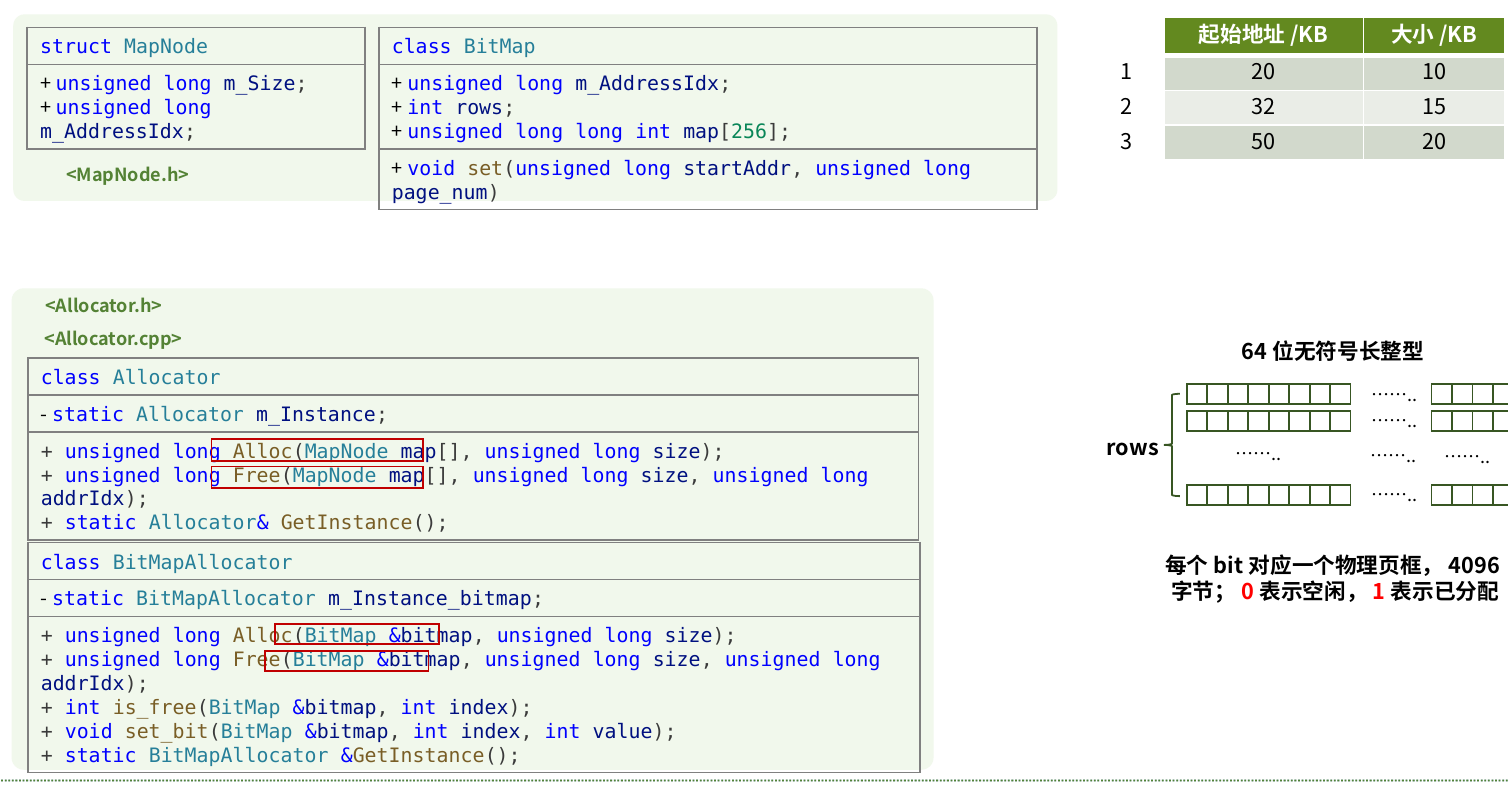
\includegraphics[width=0.9\textwidth]{figures/fig_bitmap_struct.png}
  \caption{从 MapNode 到 BitMap 的结构对比与位示图原理（图源：课程设计 PPT slide 23）}
  \label{fig:bitmap-struct}
\end{figure}

\section{bitmap 页框分配器设计}
本设计引入位示图（bitmap）作为新的页框管理结构。其核心思想是：用一个 bit 对应
一个 4KB 物理页框，0 表示空闲、1 表示已分配。由于不再要求连续，分配时只需在位示图
中找到足够数量的空闲 bit 即可，它们对应的物理页框不必相邻。\texttt{BitMap} 的定义
如下（\texttt{include/MapNode.h}，标注 NOTE 1）：

\begin{lstlisting}[caption={BitMap 位示图结构},label={lst:bitmap}]
#define M_PAGE_SIZE 4096
class BitMap
{
public:
    unsigned long m_AddressIdx;            // 本位示图管理的起始物理地址
    int rows;                              // 有效行数 (每行 64 bit)
    unsigned long long int map[256];        // 位示图本体, 256*64=16384 bit
    void set(unsigned long startAddr, unsigned long page_num)
    {
        m_AddressIdx = startAddr;
        rows = page_num / 64;
        for (int i = 0; i < rows; i++) map[i] = 0;   // 初始化为全空闲
    };
};
\end{lstlisting}

\begin{figure}[H]
  \centering
  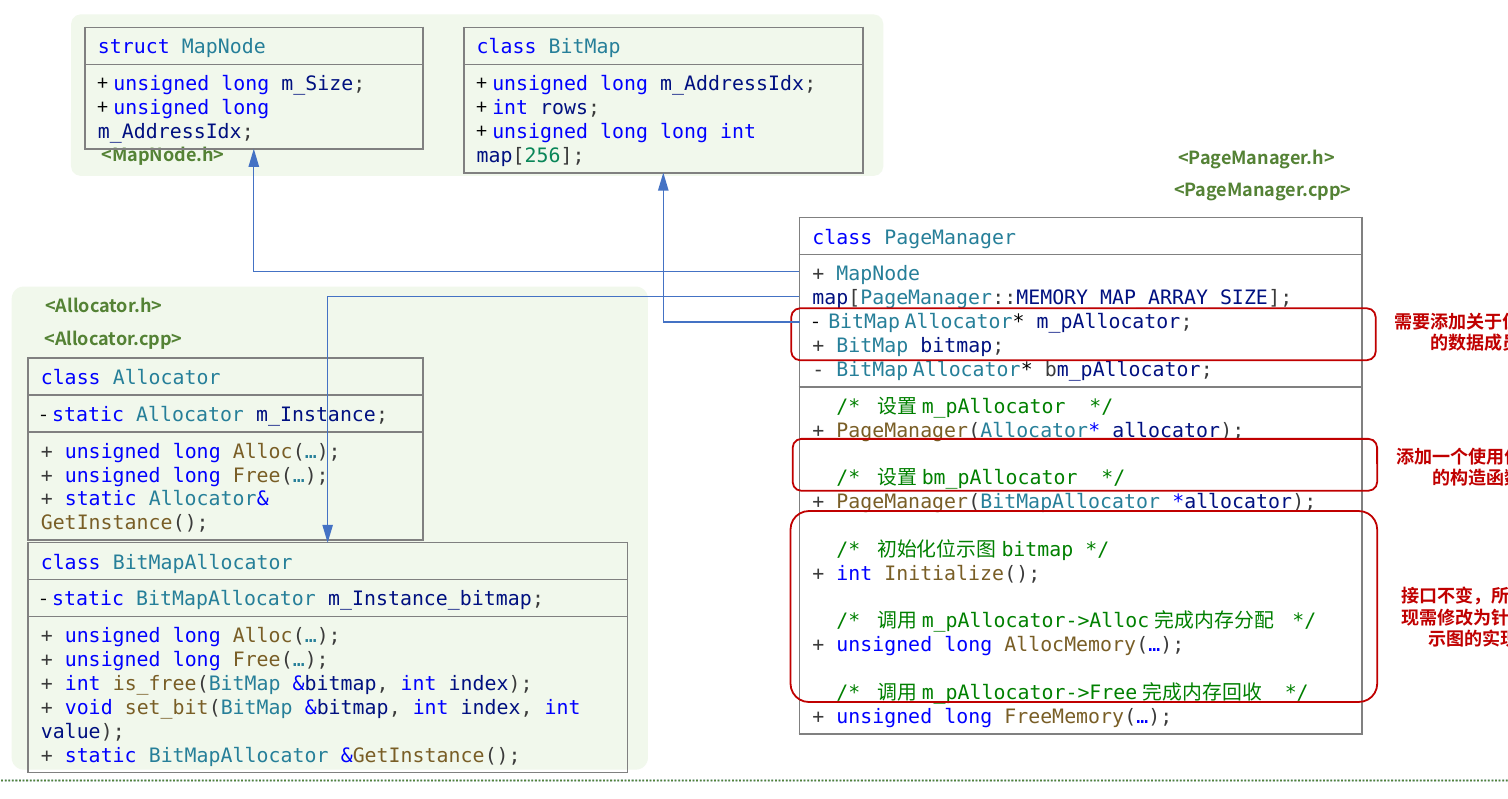
\includegraphics[width=0.9\textwidth]{figures/fig_bitmap_class.png}
  \caption{位示图管理相关的类与结构体关系（图源：课程设计 PPT slide 25）}
  \label{fig:bitmap-class}
\end{figure}

\texttt{map} 是一个 256 元素的 64 位无符号整数数组，共 $256\times 64 = 16384$ 个 bit，
最多可表示 16384 个页框，即 64MB 物理内存的页框占用情况（本设计 QEMU 配置 32MB
内存，容量充裕）。\texttt{m\_AddressIdx} 记录该位示图所管理区域的起始物理地址，
用于在位号与物理地址之间换算。

配套的分配器类 \texttt{BitMapAllocator}（\texttt{include/Allocator.h}）提供分配、
释放及位操作接口：

\begin{lstlisting}[caption={BitMapAllocator 接口},label={lst:bitmap-allocator-if}]
class BitMapAllocator
{
public:
    unsigned long Alloc(BitMap &bitmap, unsigned long size);
    unsigned long Free(BitMap &bitmap, unsigned long size, unsigned long addrIdx);
    int  is_free(BitMap &bitmap, int index);
    void set_bit(BitMap &bitmap, int index, int value);
    static BitMapAllocator &GetInstance();
};
\end{lstlisting}

\section{BitMapAllocator 的分配与释放}
\texttt{BitMapAllocator} 的分配算法在位示图中线性扫描，寻找一段连续的空闲 bit
（注意：这里要求的是\emph{位号连续}，对应物理页框在 bitmap 中编号连续，但由于
每页独立映射，物理页框是否相邻并不影响用户态连续性）。其实现见代码清单~%
\ref{lst:bitmap-alloc}。

\begin{lstlisting}[caption={BitMapAllocator::Alloc 分配算法},label={lst:bitmap-alloc}]
// 对应源码 mm/Allocator.cpp
unsigned long BitMapAllocator::Alloc(BitMap &bitmap, unsigned long size)
{
    int pages_needed = (size + M_PAGE_SIZE - 1) / M_PAGE_SIZE; // 向上取整所需页数
    int start = -1, count = 0;
    for (int i = 0; i < bitmap.rows * 64; i++)      // 扫描位示图
    {
        if (is_free(bitmap, i))                      // 第 i 位空闲
        {
            if (count == 0) start = i;               // 记录连续段起点
            if (++count == pages_needed) break;      // 找够所需页数
        }
        else count = 0;                              // 中断, 重新计数
    }
    if (count < pages_needed) return 0;              // 无足够空闲页
    for (int i = 0; i < pages_needed; i++)
        set_bit(bitmap, start + i, 1);               // 标记为已分配
    return start * M_PAGE_SIZE + bitmap.m_AddressIdx;// 返回起始物理地址
}
\end{lstlisting}

\texttt{Free} 是其逆过程：由释放地址反算起始位号，再把对应各位置 0。\texttt{is\_free}
与 \texttt{set\_bit} 是位运算原语，利用 64 位整数的位掩码完成单 bit 的读取与置位
（\texttt{map[index/64] \& (1ULL << (index\%64))}）。可以看到，整个分配器只依赖
位运算，不涉及分区表的插入、合并、搬移，实现简洁，且天然支持离散分配。

\section{内核页框池与用户页框池划分}
位示图建立之后，物理内存被划分为多个页框池，分别由不同的 \texttt{PageManager}
子类用各自的位示图管理。\texttt{PageManager}（\texttt{mm/PageManager.cpp}）在原有
\texttt{MapNode map[]} 的基础上新增了位示图成员 \texttt{bitmap} 与引用计数数组
\texttt{Page[]}，并增加了接受 \texttt{BitMapAllocator*} 的构造函数：

\begin{lstlisting}[caption={PageManager 新增的位示图与引用计数成员},label={lst:pm-members}]
// 对应源码 include/PageManager.h
class PageManager
{
public:
    MapNode map[PageManager::MEMORY_MAP_ARRAY_SIZE];
    BitMap bitmap;                                         // NOTE 1: 位示图
    int Page[MemoryDescriptor::USER_SPACE_SIZE / PAGE_SIZE]; // NOTE 3: 页引用计数
private:
    BitMapAllocator *m_pAllocator;
    unsigned long AllocMemory(unsigned long size);         // 调用 m_pAllocator->Alloc
    unsigned long FreeMemory(unsigned long size, unsigned long startAddress);
};
\end{lstlisting}

两个子类分别划定各自的管理范围。\texttt{KernelPageManager} 管理页表区中除固定占用
部分（页目录、核心页表、0\# 用户页表共占 4 页）之外的剩余页框，其起始地址定义为
\texttt{0x200000 + 0x2000 + 0x2000 = 0x204000}，大小为
\texttt{0x200000 - 0x4000}；\texttt{UserPageManager} 则管理从 \texttt{0x400000}
（4M）起至整个物理内存末端的用户区。两者在 \texttt{Initialize()} 中分别调用
\texttt{bitmap.set(...)} 把各自范围初始化为全空闲：

\begin{lstlisting}[caption={用户页框池的位示图初始化},label={lst:user-pm-init}]
// 对应源码 mm/PageManager.cpp :: UserPageManager::Initialize
this->map[0].m_AddressIdx = USER_PAGE_POOL_START_ADDR / PageManager::PAGE_SIZE;
this->map[0].m_Size       = USER_PAGE_POOL_SIZE / PageManager::PAGE_SIZE;
this->bitmap.set(USER_PAGE_POOL_START_ADDR, USER_PAGE_POOL_SIZE / PageManager::PAGE_SIZE);
\end{lstlisting}

需要强调的是，bitmap 只管理"可动态分配"的页框池；内核映像本身、页目录及固定页表
所占用的页框是静态固定的，不在 bitmap 的动态分配范围之内，因此不会与之冲突。

\section{页引用计数机制}
仅有位示图还不够。写时复制（COW）与正文段共享都允许多个进程的页表项指向同一个
物理页框，因此一个物理页是否能够真正释放，不能只看某一个页表项，而要看它是否还被
其他进程引用。为此，\texttt{PageManager} 引入了页引用计数数组 \texttt{Page[]}，
其长度为用户空间大小除以页大小（\texttt{USER\_SPACE\_SIZE / PAGE\_SIZE}），
\texttt{Page[i]} 记录第 \texttt{i} 个用户区物理页框的共享份数。

引用计数与分配、释放逻辑紧密耦合（\texttt{mm/PageManager.cpp}）：

\begin{lstlisting}[caption={带引用计数的分配与释放},label={lst:page-refcount}]
unsigned long PageManager::AllocMemory(unsigned long size)
{
    unsigned long newaddr = this->m_pAllocator->Alloc(this->bitmap, size);
    Page[newaddr >> 12] = 1;                       // 新分配页, 引用计数置 1
    return newaddr;
}
unsigned long PageManager::FreeMemory(unsigned long size, unsigned long startAddress)
{
    Page[startAddress >> 12]--;                     // 引用计数减一
    if (Page[startAddress >> 12] == 0)              // 无人再引用, 才真正释放
        this->m_pAllocator->Free(this->bitmap, size, startAddress);
    return 1;
}
\end{lstlisting}

\texttt{AllocMemory} 在分配后立即把对应页的引用计数置为 1；\texttt{FreeMemory}
则\emph{先}把引用计数减一，只有当计数归零时才调用底层的 \texttt{BitMapAllocator::Free}
真正归还页框。配合 \texttt{fork} 时对共享页的 \texttt{Page[]++}（见第五章），物理页的
生命周期便由引用计数而非单个页表项统一管理，这正是 COW 与 text 共享得以正确释放的
关键。

\section{KernelAllocator 的同步适配}
值得说明的是，位示图改造集中在 \texttt{PageManager} 体系（页表区与用户区），而
管理内核堆对象区的 \texttt{KernelAllocator} 仍沿用原有的连续分区方式——它依旧
持有 \texttt{MapNode map[]} 并通过旧的 \texttt{Allocator::Alloc/Free} 进行分配，
管理从 \texttt{0x180000}（1.5M）起的 512KB 内核堆（\texttt{include/KernelAllocator.h}）。

这一"不改"本身就是一种经过权衡的取舍：内核堆对象多为变长的小对象（如各种内核数据
结构的动态实例），连续分区的变长分配对这类场景更为合适；而位示图以页框为最小单位，
更适合页表、用户图像这类按页分配的对象。因此本设计让两者并存：\texttt{KernelAllocator}
保持兼容以服务内核堆，\texttt{KernelPageManager}/\texttt{UserPageManager} 则全面转向
位示图以服务页框级分配。这种分工使得改造得以聚焦于真正需要离散化的部分，避免对内核
堆对象管理做不必要的、风险更高的改动。

\subsection*{运行验证}
为验证位示图分配在运行时的正确性，在 shell 中执行 \texttt{/bin/malloc} 与
\texttt{/bin/stack} 两个用户程序。\texttt{malloc} 输出 \texttt{test of malloc}，
表明用户态堆分配（经内核堆对象区的分配管理）正常工作（图~\ref{fig:run-malloc}）；
\texttt{stack} 程序递归压栈、输出由大到小的计数，验证了离散页表下栈页能够按需扩展
分配（图~\ref{fig:run-stack}）。两者共同说明位示图分配能够支撑用户态堆栈的动态增长。

\begin{figure}[H]
  \centering
  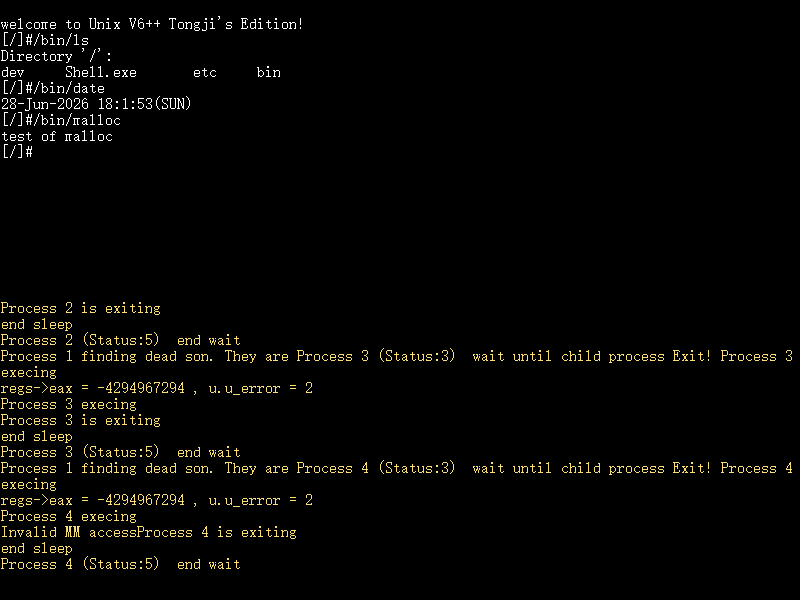
\includegraphics[width=0.85\textwidth]{figures/run_malloc.png}
  \caption{运行 /bin/malloc：用户堆分配测试}
  \label{fig:run-malloc}
\end{figure}

\begin{figure}[H]
  \centering
  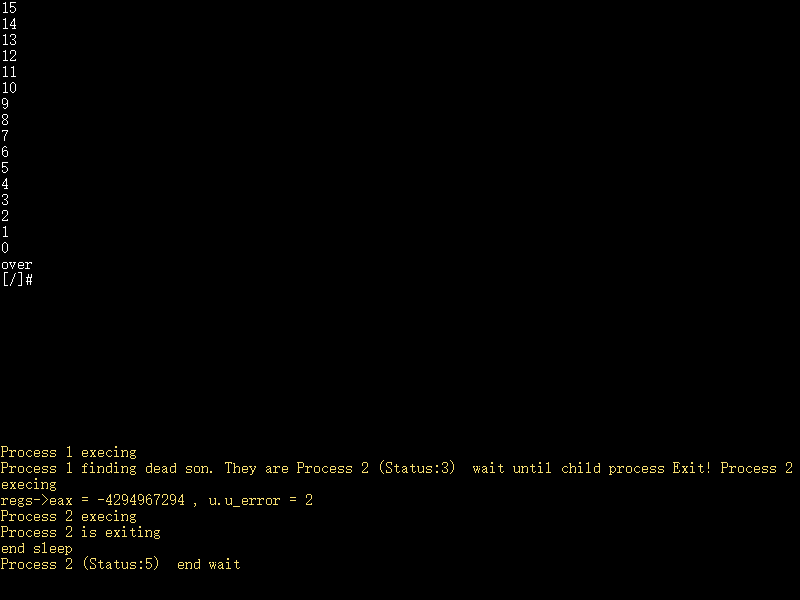
\includegraphics[width=0.85\textwidth]{figures/run_stack.png}
  \caption{运行 /bin/stack：离散页表下栈按需扩展}
  \label{fig:run-stack}
\end{figure}

\section{本章小结}
本章把物理页框的分配方式从连续空闲分区表改造为位示图。\texttt{BitMap} 以每页一个
bit 的粒度记录页框占用，\texttt{BitMapAllocator} 通过位运算完成离散分配与释放；
页表区与用户区分别由 \texttt{KernelPageManager}/\texttt{UserPageManager} 用各自的
位示图管理；\texttt{Page[]} 引用计数则与分配/释放逻辑耦合，为共享物理页的生命周期
管理提供依据。这一层改造与第三章的页表改造共同构成了离散化进程映像管理的物理基础。
